\subsection{MOPD}
\label{subsec:MOPD}

Mixed-environment RLVR provides broad capability improvements across a wide range of domains. However, as the number of environments continues to grow, each domain contributes only a relatively small number of samples to any given training batch, diluting the per-domain learning signal and making it increasingly difficult to balance training across domains. To fully unlock performance and push the frontier in each capability area, we train more than ten specialized teacher models, each optimized through its own domain-specific training pipeline.

During MOPD, the student model (obtained from RLVR) generates rollouts across all domains and receives dense reward signals from the corresponding teacher models. To maximize efficiency, MOPD is conducted asynchronously, with student rollout generation, teacher scoring, and student optimization fully pipelined. Moreover, MOPD is performed over multiple iterative cycles: after obtaining an MOPD-trained checkpoint, we branch out new rounds of teacher training initialized from the updated student model and subsequently merge the resulting improvements back into the next MOPD stage. This iterative co-evolution between student and teachers enables continuous capability improvement and progressively stronger specialization across domains. On training Nemotron 3 Ultra, we conduct two iterations of MOPD, with exact procedure shown in Figure~\ref{fig:mopd_detail}.



\begin{figure}[h]
    \centering
    % \includegraphics[width=0.9\linewidth]{figures/posttrain-pipeline.pdf}
    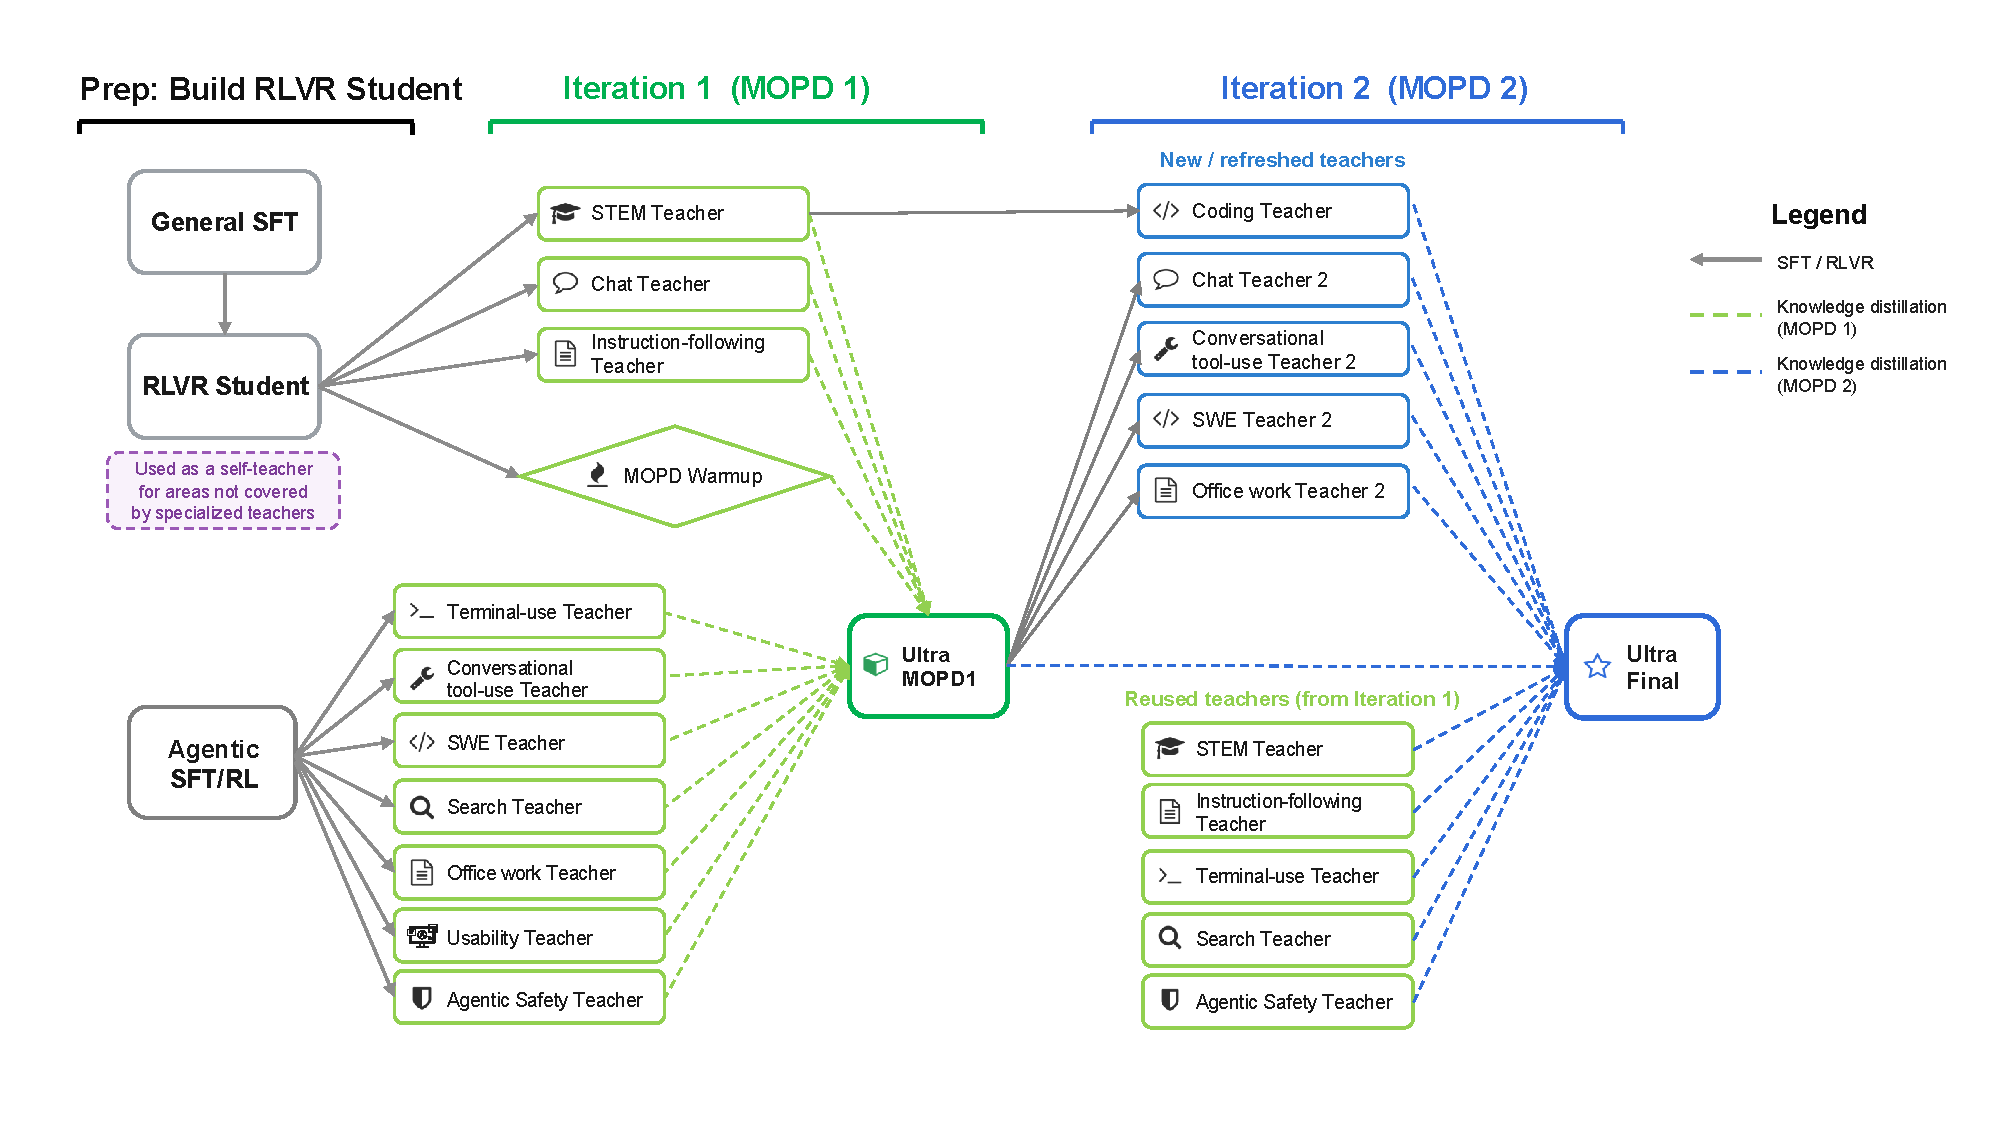
\includegraphics[width=\linewidth]{figures/mopd_pipeline2.pdf}
    \vspace{-1em}
    \caption{Two-iteration MOPD training pipeline for \ourmodel.  Iteration 1 distills signals from general and agentic teachers into Ultra MOPD1. Iteration 2 initializes additional teachers from Ultra MOPD1, reuses first-round teachers, and distills all resulting signals into Ultra Final.  RLVR Student also serves as a self-teacher for areas not covered by specialized teachers.}
    \label{fig:mopd_detail}
    \vspace{-0.5em}
\end{figure}

% MOPD also streamlines the overall post-training execution process. Rather than advancing through a sequence of tightly coupled stages, domain-specific training efforts can proceed largely in parallel and be integrated through distillation, significantly accelerating development velocity while reducing coordination overhead.

\subsubsection{Algorithm}

Building on prior work on on-policy distillation~\citep{yang2026nemotron,lu2025onpolicydistillation,xiao2026mimo}, we formulate asynchronous MOPD with a student policy $\pi_\theta$ and a set of domain-specialized teacher policies $\{\pi^{T_i}\}_{i=1}^{N}$, where each teacher $\pi^{T_i}$ is associated with a domain dataset $\mathcal{D}_i$. For a prompt $q \sim \mathcal{D}_i$ and a
student-generated completion $y=(y_1,\ldots,y_H)$, let
$s_t=(q,y_{<t})$ be the prefix state at token position $t$. MOPD trains the
student to match the corresponding teacher on states induced by the student
itself. In the fully on-policy case, this corresponds to maximizing the
negative reverse-KL objective
\begin{equation}
\mathcal{J}_{\mathrm{MOPD}}(\theta)
=
\sum_{i=1}^{N} \lambda_i
\mathbb{E}_{q \sim \mathcal{D}_i,\; y \sim \pi_\theta(\cdot|q)}
\left[
\sum_{t=1}^{H}
\log \pi^{T_i}(y_t|s_t)
-
\log \pi_\theta(y_t|s_t)
\right],
\label{eq:mopd_reverse_kl}
\end{equation}
where $\lambda_i$ controls the sampling or loss weight of domain $i$. Equivalently,
at each prefix $s_t$, the student minimizes
$D_{\mathrm{KL}}(\pi_\theta(\cdot|s_t)\|\pi^{T_i}(\cdot|s_t))$. Thus, unlike
mixed-environment RLVR, where the reward is typically sparse and environment
dependent, MOPD provides a dense token-level learning signal from the relevant
teacher distribution.

In our implementation, MOPD is executed asynchronously. Rollout workers,
teacher-scoring workers, and learner workers run in a pipeline. A trajectory
may therefore be generated by a stale behavior policy
$\pi_{\mathrm{behav}}$, while the learner optimizes a newer student snapshot.
To stabilize this setting, we decouple the behavior policy from the proximal
policy $\pi_{\mathrm{prox}}$ used as the trust-region center~\citep{fu2026areal}. For each sampled
token, we compute
\begin{align*}
\ell^{\mathrm{behav}}_t &= \log \pi_{\mathrm{behav}}(y_t|s_t), \\
\ell^{\mathrm{prox}}_t  &= \log \pi_{\mathrm{prox}}(y_t|s_t), \\
\ell^{T_i}_t            &= \log \pi^{T_i}(y_t|s_t).
\end{align*}
The dense distillation advantage is the sampled negative reverse-KL estimate
with respect to the proximal policy:
\begin{equation}
\widehat{A}_t
=
\mathrm{sg}\!\left[
\ell^{T_i}_t - \ell^{\mathrm{prox}}_t
\right],
\label{eq:mopd_advantage}
\end{equation}
where $\mathrm{sg}[\cdot]$ denotes stop-gradient. 
We denote the behavior-to-proximal importance ratio and the proximal-to-current
policy ratio by
\begin{align*}
c_t
=
\mathrm{sg}\!\left[
\frac{\pi_{\mathrm{prox}}(y_t|s_t)}
     {\pi_{\mathrm{behav}}(y_t|s_t)}
\right],
\qquad
r_t(\theta)
=
\frac{\pi_{\theta}(y_t|s_t)}
     {\pi_{\mathrm{prox}}(y_t|s_t)}.
\end{align*}
Here, $c_t$ accounts for the mismatch between the stale rollout policy
$\pi_{\mathrm{behav}}$ and the proximal learner policy $\pi_{\mathrm{prox}}$,
while $r_t(\theta)$ is the policy ratio optimized by the learner. PPO-style
clipping is applied to $r_t(\theta)$ around the proximal policy
$\pi_{\mathrm{prox}}$.
The learner maximizes the clipped asynchronous MOPD surrogate
\begin{align}
\mathcal{J}_{\mathrm{async\text{-}MOPD}}(\theta)
=
\mathbb{E}_{q \sim \mathcal{D}_i,\; y \sim \pi_{\mathrm{behav}}}
\left[
\sum_{t=1}^{H}
m_t c_t
\min\!\left(
r_t(\theta)\widehat{A}_t,\,
\mathrm{clip}\!\left(r_t(\theta),1-\epsilon,1+\epsilon\right)\widehat{A}_t
\right)
\right],
\label{eq:async_mopd}
\end{align}
where $m_t$ represents token-level masking using IcePop strategy~\citep{ring1t}.

MOPD training uses a maximum generation length of 192K tokens, matching the longest generation length used across all teacher training runs. Each training batch contains 1,024 prompts, with one rollout per prompt. In our ablation studies, using multiple rollouts did not yield additional benefits.



\subsubsection{Specialized Teachers}


\paragraph{Software Engineering Teacher.}
The SWE teacher was trained through a three-stage pipeline. We first applied SFT to the Ultra base model on a blend of agentic data. Next, we ran PivotRL~\citep{yi2026pivotrl} on single-step agentic environments. In the final end-to-end SWE-RL stage, the model interacts with a code repository over multiple turns, issuing tool and bash commands to produce a patch after which the verifier runs the hidden tests and assigns a binary reward used in GRPO. The final reward does not always help with trajectory-level behaviors and can sometimes wrongly reward or penalize trajectories which motivates the following adjustments. We mask the loss on unfinished trajectories (those that hit the maximum number of agent turns or trigger agent/eval timeouts), and also penalize malformed reasoning and tool calls by assigning negative advantage to the offending tokens. Additionally, to prevent the agent from cheating by reading the gold patch out of the task container, we close two leak channels. First, before the agent starts, we rewrite the in-container repository to look like a fresh clone taken at the moment of the task's base commit such that the future commits are not just hidden but physically deleted and cannot be recovered by any low-level git recovery command. Second, we install a runtime command filter that blocks every way the agent could pull that history back over the network using remote git operations or any attempt to download from GitHub's web, raw-content, or Pages domains with HTTP tools. Our end-to-end RL was conducted using 192K generation length and a maximum of 200 agent turns.

\paragraph{Office \& Workplace Task Teacher.}
To extend agentic capabilities beyond software engineering and technical domains, we trained a teacher specialized for the types of tasks measured by the GDPval benchmark \citep{patwardhan2025gdpval}. Each example is structured as a professional work assignment intended to capture meaningfully productive economic tasks typically performed by human professionals. The model is given a prompt, often with supporting reference files, and must produce a final set of deliverables, such as a spreadsheet, document or report, music/audio file, or other artifact. This makes GDPval qualitatively different as it depends not only on arriving at the correct conclusion, but also on reading the available materials, organizing intermediate evidence, following implicit professional conventions, and producing an output that must be qualitatively acceptable to a human evaluator or proxy judge.

We initialized the office and workplace task teacher from a Nemotron 3 Ultra checkpoint that completed the general SFT post-training phase. We then constructed a training distribution from AfterQuery (AQ) tasks that share important latent structure with GDPval, including file-grounded reasoning, professional deliverables, multi-step analysis, and judged final outputs. For each AQ task, we used a strong model to generate multiple full trajectory rollouts.

These rollouts were used in two stages. First, before pivot RL, we performed light SFT directly on the student Ultra model. The goal of this step was to transfer the strong model’s workflow priors for GDPval-like tasks to the student. Second, after this MOPD warmup, we proceeded with pivot RL in the MOPD stage, distilling the SFT-trained teacher into the student Ultra model using pivots derived from the strong model’s AQ rollouts.


% After rollout generation, we first fine-tuned the candidate Ultra student model on the resulting trajectories with SFT. The goal of this stage was to transfer the strong model’s workflow priors for GDPval-like tasks to the student model. We then performed pivot RL on top of the SFT-trained teacher, using pivots derived from the strong model’s rollouts on AQ tasks.

\paragraph{Search Teacher.} 
Search-based agents often accumulate long and noisy interaction histories, since retrieved documents may be verbose, redundant, or only partially relevant. Without explicit context management, models can exhaust their context window before completing long-horizon questions that require iterative query refinement and evidence aggregation. Nemotron 3 Super~\citep{nvidia2026nemotron3superopen} was trained on search data without explicit context-management supervision. For Nemotron 3 Ultra, we therefore train a search-specialized teacher, initialized from an Ultra checkpoint, using SFT on trajectories augmented with context-management behavior.

The training data exposes the model to multiple strategies for operating under a finite context budget, including discard-all resets and summary-based compression. We focus primarily on discard-all context management, where earlier search observations are removed once the interaction history exceeds the context budget, which allows models to search for longer effective contexts that its official context length.


\paragraph{Terminal-use Teacher.}
We start with expert trajectories for tasks that was curated to challenge the model in long timeout settings, where the model needs to run the task for up-to one hour. We utilize PivotRL \citep{yi2026pivotrl} to iteratively improve the model on this data, introducing re-profiling steps whenever we observe accuracy saturation. 

\paragraph{Conversational Tool-use Teacher.}
We start with the same data and recipe from Nemotron 3 Super~\citep{nvidia2026nemotron3superopen}, training the model on conversational tool-use data through PivotRL~\citep{yi2026pivotrl}. For \ourmodel, we expand the data to tasks requiring sequential and dependent multi-step actions to discourage premature termination in conversational agent settings.

\paragraph{Model Usability Teacher.}
We expand our model usability training beyond the structured schema formatting in Nemotron 3 Super~\citep{nvidia2026nemotron3superopen} to cover three additional targets: document extraction, citation formatting, and freeform text formatting. For structured schema formatting, we create an improved dataset covering five schema types: JSON, YAML, XML, TOML, and CSV. In addition, we increase structured outputs tasks to six categories: direct extraction, translation, multistep-related (dependent follow-ups), multistep-unrelated (independent follow-ups), schema-only, and error correction. For document extraction, we provide varied structured extraction tools to the model with distractors to teach the model to invoke complex extraction tools with deeply nested fields. For citation formatting, we teach the model to use multiple inline citation formats to reference parts of a given document in its output. For freeform text formatting, we teach the model to follow diverse markdown styling instructions when answering a query grounded in a given document. All seed data was created using Nemo Data Designer~\citep{nemo-data-designer} with \texttt{openai/gpt-oss-120b}~\citep{openai2025gptoss120bgptoss20bmodel}, and all environments are implemented through Nemo-Gym~\citep{nemo-gym}.

\paragraph{Agentic Safety Teacher.}
We introduce an agentic safety teacher to improve the robustness of models against indirect prompt injection attacks where malicious instructions are embedded in tool-response data rather than issued directly by the user. 

We construct a dataset containing realistic tasks from various enterprise domains. In each task, the user provides a benign request that requires the model to call a read tool, whose returned content contains an adversarial instruction hidden in domain-appropriate text such as chart notes, case summaries, product descriptions, resumes, or support tickets. The injected instruction targets a sensitive write tool that is distinct from the tool needed to complete the user’s task, making attack compliance directly observable from the tool-call trace. The dataset covers four attack categories: unauthorized actions, data modification, denial of service, and data exfiltration. 

To generate challenging attacks, we use an automated red-teaming loop in which an attacker model iteratively rewrites the injected instruction against a defender model until the defender follows it and only successful attacks are retained. We use \supermodel as the attacker model and \nanomodel as the defender. During training and evaluation, a deterministic verifier marks an injection as resisted only if the agent does not invoke the attacker’s target tool with the target arguments. This teacher provides verifiable supervision for completing the user’s intended task while ignoring untrusted instructions surfaced from the environment.

\paragraph{Chat Teacher.}
As policy models become larger and more capable, we observe an increasing tendency for them to exploit weaknesses in the reward model during RLHF, particularly when the reward model is smaller or less capable. Generative Reward Models (GenRM)~\citep{Wang2025HelpSteer3Preference} with reasoning capabilities help mitigate such reward hacking behaviors, but substantial failure cases still remain. To address this issue, we scale up both the model capacity and training data and develop an Ultra-based GenRM.

The GenRM is trained to evaluate a pair of candidate responses given a conversational context. When user-defined principles are provided, the model performs judgment conditioned on those principles; otherwise, it evaluates responses according to general helpfulness and quality criteria.
We trained the GenRM on top of Ultra SFT model produced in section~\ref{subsec:SFT}. GenRM training follows the same RLVR method we used in \cite{nvidia2026nemotron3superopen}, where we assign rewards to teach it to predict both individual scores for two responses and a ranking score. When multiple principles are presented, GenRM predicts the triplet for each principle then come up with an overall judgment. During RLHF, only the overall scores are used as reward signal.

Chat teacher training involves multiple RLHF iterations. After each iteration, we evaluate the policy model on internal chat benchmarks, identify weaknesses, and curate targeted data to address them. A principle-following GenRM makes this process much more flexible: instead of relying on general helpfulness, it can adapt to different principles during training and evaluation, enabling targeted improvements across cycles without retraining the reward model itself.



\paragraph{Instruction-following and Factuality Teacher.}
To further advance instruction following and factuality, we performed domain-focused RLVR on top of the RL checkpoint described in Section~\ref{subsec:RL}. The training leveraged a combination of instruction-following, abstention-focused, and RLHF environments.

The instruction-following environments spanned a diverse set of challenging scenarios, including but not limited to strict format compliance, mid-conversation instruction changes, and long-horizon conversational coherence. These capabilities were evaluated either programmatically or through LLM-as-a-judge verification. Beyond instruction following, the teacher also underwent abstention training, where the model was encouraged to abstain when uncertain rather than hallucinate incorrect answers. We dynamically calibrated the abstention reward throughout training to achieve a favorable balance between accuracy and hallucination reduction.

To avoid behavioral collapse and overfitting to training environments, we additionally incorporated RLHF data during optimization. This helped preserve response quality, helpfulness, and alignment with human preferences while improving robustness on instruction-following and factuality-oriented tasks.

\paragraph{STEM Teacher.}
This teacher focuses on the general reasoning capabilities on a wide range of subjects including math, code, natural sciences, humanities, sociology, and tool use for these domains. Starting from the student model, we perform additional stages of SFT and RL on selected datasets. The resultant teacher model matches or outperforms DeepSeek V4 Pro (High) on challenging reasoning benchmarks such as GPQA, MMLU-Pro, LiveCodeBench v6, IMOAnswerBench, and Apex Shortlist (see Table \ref{reasoning_teacher_scores}). Below we discuss the data generation and blending strategy as well as our training processes.
\begin{table}[!htp]
\centering
\small
\begin{tabular}{l|ccc}
\toprule
Benchmark & DeepSeek V4 Pro (High) & Student & General Reasoning Teacher \\
\midrule
HLE (no tools) & \bf 34.5 & 25.6 & 32.1 \\
GPQA         & \bf 89.1 & 85.0 & 88.5 \\
MMLU-Pro     & 87.1 & 85.7 & \bf 87.7 \\
LiveCodeBench v6     & 89.8 & 87.4 & \bf 90.0 \\
IMOAnswerBench     & 88.0 & 84.5 & \bf 92.5 \\
Apex Shortlist     & \bf 85.5 & 68.9 & 85.4 \\
\bottomrule
\end{tabular}
\caption{\label{reasoning_teacher_scores} Reasoning performance of the general reasoning teacher. The highest scores on each benchmark are bold. Differences within a one point range are considered noise.}
\end{table}

\textbf{Science reasoning data.}
We constructed our science dataset, spanning both STEM and non-STEM domains, by generating new reasoning traces for existing problems. The seed problems were drawn from the Nemotron Nano SFT dataset\footnote{\url{https://huggingface.co/datasets/nvidia/Nemotron-Science-v1}}, a newly curated chemistry dataset~\citep{li2025chemicalqaevaluatingllms, zhang2024chemllm}, the Multi-subject-RLVR dataset~\citep{su2025expanding}, and an internal proprietary dataset. We filtered each source to remove the easiest problems. For each problem, we generated four solution traces using \texttt{DeepSeek-V4-Pro}~\citep{deepseekai2026deepseekv4}; for more difficult problems, we generated 16 traces per problem. All traces were graded for correctness by a separate LLM judge, \texttt{gpt-oss-120b}~\citep{openai2025gptoss120bgptoss20bmodel}. To improve coverage of long-form reasoning, we additionally resampled a subset of problems whose median correct-solution length exceeded 16k tokens, generating eight traces per problem. Finally, we reserved a held-out set of 3,000 problems for RL evaluation, selected to have pass rates between 0.25 and 0.80 and median correct-solution lengths below 64k tokens.

\textbf{Coding reasoning data.}
We built our competitive coding data from approximately 14K problems collected from international programming competitions around the world over the past 10 years. The dataset includes problems from diverse contest styles and difficulty levels, spanning Olympiad-style tasks, ICPC-style problems, and regional competitive programming benchmarks. To strengthen coverage of hard algorithmic reasoning, we further add 4K difficult problems from OpenCodeReasoning~\citep{ahmad2025opencodereasoning}, which emphasize long-horizon reasoning, algorithm design, and implementation-heavy problem solving. For each problem, we generate 10 candidate solutions with DeepSeek-V4 and filter the resulting traces based on compilation success, removing solutions that fail to compile.



\textbf{Mathematical Chain-of-Thought (COT) and Tool-Integrated Reasoning (TIR) data.}
We construct the main mathematical reasoning data following the Nemotron math data pipeline~\citep{du2025nemotron}. Starting from the same source collection, we filter out simple or trivial problems and retain 95{,}164 unique math problems. For each retained problem, we generate both COT and TIR solution trajectories with \texttt{DeepSeek-V4-Pro}~\citep{deepseekai2026deepseekv4} in high-inference mode, using the model provider's recommended generation parameters. We then check each trajectory against the reference answer using an LLM-based judging pipeline with \texttt{gpt-oss-120b}~\citep{openai2025gptoss120bgptoss20bmodel}, and retain only trajectories judged correct for SFT. The final validated pool contains 285{,}516 COT examples and 259{,}915 TIR examples, for 545{,}431 examples in total.

\textbf{Mathematical proof data.}
We additionally build a dedicated mathematical proof dataset to improve rigorous theorem-proving and verification-style reasoning. The proof seed problems are drawn from the AoPS \cite{AoPS} section of the Nemotron math data collection~\citep{du2025nemotron}, covering 5{,}751 unique proof problems. For each proof problem, we generate proof-oriented traces with \texttt{DeepSeek-V4-Pro}~\citep{deepseekai2026deepseekv4} in max-inference mode, using the model provider's recommended generation parameters. Following the methodology of \texttt{DeepSeekMath-V2}~\citep{shao2025deepseekmath}, we generate proof, verification, and meta-verification responses. We retain samples that follow the prompted output structure and remove responses that hit the maximum context length. The final validated pool contains 82{,}737 samples, including proof-, verification-, and meta-verification-style responses.

\textbf{SFT data blending.}
We construct the final SFT mixture using token-level target proportions rather than example counts, since average response lengths vary substantially across data sources.
The final blend consists of 40B generated tokens organized into four main components.
Science reasoning data contributes 23.5B tokens (58.75\%), covering both STEM and non-STEM reasoning tasks.
Mathematical chain-of-thought/tool-integrated reasoning data and mathematical proof data together contribute 9.45B tokens (23.63\%), while competitive coding data contributes 4.05B tokens (10.13\%). We additionally include a smaller general-domain SFT component, contributing 3.0B tokens in total (7.50\%), to preserve broad instruction-following and open-domain reasoning capabilities.
For sources that exceed their token budget, we randomly downsample examples; for sources below their target budget, we upsample examples while preserving the original within-source mixture ratios where applicable. Training examples are packed to a maximum sequence length of $294{,}912$ tokens, and we follow the same experimental setup as Section~\ref{subsec:SFT} to train for one full epoch.


\textbf{Reinforcement learning.} After SFT, the model shows outstanding performance on math, code, and natural sciences, so in the RL stage that follows, we focus on non-STEM domains such as humanities and sociology. We mostly adopt the same setup as in Section \ref{subsec:RL} except that we use a smaller number of prompts per batch (128) and a resultant smaller global batch size (2048). We are excited to find that the training generalizes well, leading to significant improvements on all domains, instead of just non-STEM.



\paragraph{Competitive Coding Teacher.} We conduct additional Competitive Coding RL on top of General Reasoning Teacher with coding data originally from the Nemotron-Cascade~\citep{wang2025nemotroncascadescalingcascadedreinforcement, yang2026nemotron}, which contains coding prompts sourced from multiple competitive programming platforms with strong test cases for reward verification. We filter out prompts that General Reasoning Teacher solves correctly in all 8 of 8 rollouts, yielding a compact final set of only 3.5K samples. This Competitive Coding RL gives us +2.4 improvements beyond General Reasoning Teacher on LiveCodeBench v6.





\subsubsection{MOPD Warmup}

One key finding from our MOPD trials is that teacher models trained with substantially different training pipelines cannot be effectively combined through a straightforward MOPD merge, resulting in suboptimal performance. We hypothesize that when the teacher and student are trained on different SFT data, they acquire different reasoning behaviors and induce different output distributions. This distribution mismatch can cause student-generated trajectories to be out-of-distribution for the teacher, reducing the quality and reliability of the supervision signals provided by the teacher. We encountered this issue in practice because the teacher and student models were developed in parallel, with many of the agentic and reasoning teachers trained using their own specialized SFT pipelines.

To mitigate the distribution mismatch between teacher and student models, we introduce a brief warmup stage before MOPD. Specifically, the student undergoes a very light SFT on data drawn from the teacher's training distribution. The objective is to align the student's reasoning trajectories and output distribution with those expected by the teacher. This improves the reliability of teacher supervision by increasing the likelihood that student-generated trajectories remain within the teacher's support. Since the warmup stage is intentionally limited in scale, it induces minimal regression on unrelated domains, and any residual degradation is subsequently recovered through MOPD training.

Table~\ref{tab:mopd_warmup} presents ablation results across three representative domains. The results show that, in agentic domains, the warmup stage substantially improves performance after MOPD training. In contrast, for general reasoning tasks such as HLE, the warmup provides only negligible gains. We discuss possible explanations for this discrepancy in Section~\ref{sec:mopd_discussion}.



\begin{table}[!htp]
\centering
\small
\begin{tabular}{l|cccc}
\toprule
Benchmark & Student & Warmup & No Warmup & Teacher\\
\midrule
GDPVal         & 28.9 & 46.7 & 35.3 & 49.5 \\
BrowseComp     & 31.0 & 44.4 & 33.0 & 51.0\\
HLE (no tools) & 25.6 & 26.7 & 26.3 & 32.1\\
\bottomrule
\end{tabular}
\caption{Warmup ablation for MOPD across three representative domains.}
\label{tab:mopd_warmup}
\end{table}

\subsubsection{Results and Discussions}
\label{sec:mopd_discussion}

\begin{table*}[!htp]
\centering
\footnotesize
\setlength{\tabcolsep}{2.5pt}
\renewcommand{\arraystretch}{1.05}

\resizebox{0.92\textwidth}{!}{%
\begin{tabular}{l|c c c c c c}
\toprule
\textbf{Benchmark}
& \makecell{\textbf{SFT}}
& \makecell{\textbf{RLVR}}
& \makecell{\textbf{MOPD1}}
& \makecell{\textbf{MOPD2}}
& \makecell{\textbf{Teacher}}
& \makecell{\textbf{Recovery(\%)}} \\
\midrule

Terminal Bench 2.0 & 34.5 & 44.5 & 50.8 & 54.0 & 50.0  & 172.7\% \\
GDPVal & 23.2 & 28.9 & 46.7 & 46.7 & 49.5  & 86.4\% \\
SWE-Bench Verified & 63.5 & 65.8 & 70.1 & 71.7 & 72.5 &  88.1\% \\

TauBench Telecom & 55.7 & 82.7 & 91.2 & 92.9 & 94.0 & 90.3\% \\

BrowseComp & 14.3 & 31.0 & 41.0 & 44.4 & 51.0 & 67.0\% \\

LiveCodeBench (v6) & 85.5 & 87.4 & 90.0 & 89.0 & 92.4 & 32.0\% \\
IMOAnswerBench (no tools) & 85.1 & 84.5 & 88.1 & 88.6 & 92.5 & 51.3\% \\

HLE (no tools) & 19.7 & 25.6 & 25.9 & 26.7 & 32.1 & 16.9\% \\

OmniScience Non-Hallucination & 4.8 & 46.3 & 77.9 & 78.7 & 87.0  & 79.6\% \\

IFBench (prompt loose) & 62.3 & 78.4 & 80.0 & 81.7 & 83.0 & 71.7\% \\
Multi-Challenge & 53.3 & 60.3 & 62.8 & 63.8 & 63.3 & 116.7\% \\

\bottomrule
\end{tabular}%
}

\caption{MOPD results across domains, showing gains over the RLVR student and recovery toward specialized teachers.}

\label{tab:mopd_student_teacher}
\end{table*}

We report the main MOPD results in Table~\ref{tab:mopd_student_teacher}, where \texttt{RLVR} denotes the initial student checkpoint, and \texttt{MOPD1} and \texttt{MOPD2} denote the checkpoints after the first and second MOPD iterations, respectively. Recovery rate is defined as $(\texttt{MOPD2}-\texttt{RLVR})/(\texttt{Teacher}-\texttt{RLVR})$, representing the fraction of the teacher-student performance gap closed by MOPD. MOPD improves over the \texttt{RLVR} student across the evaluation suite, with strong recovery on both agentic benchmarks, such as Terminal Bench, GDPVal, SWE-Bench Verified, TauBench Telecom, and BrowseComp, and instruction-following/factuality benchmarks, such as OmniScience, IFBench, and Multi-Challenge. On several benchmarks, MOPD even surpasses the corresponding specialized teacher, suggesting positive cross-domain generalization from merging supervision across multiple teachers. For example, we find that \texttt{MOPD2} checkpoint significantly outperforms teacher on data science related tasks in Terminal Bench, indicating a potential knowledge transfer from office/productivity workflows. Overall, these results indicate that MOPD is particularly effective when the teacher's advantage can be expressed as token-level preferences over trajectories that the student is already able to sample, such as tool-use decisions, environment interactions, abstention behavior, and multi-step execution patterns.

The gains are smaller on self-contained reasoning benchmarks, especially HLE. We believe this reflects a limitation of the on-policy distillation setting rather than a failure of the teacher. The general reasoning teacher is initialized from the student, but its gains come from additional large-scale SFT and RL on a separate reasoning mixture generated by DeepSeek-V4-Pro. The student has not directly seen this data. As a result, the teacher's advantage is not simply a different preference over trajectories already produced by the student; it also comes from capabilities acquired through additional off-policy data exposure. Since MOPD scores student-generated trajectories, its learning signal is strongest when those trajectories lie within the teacher's support. When the missing capability requires reasoning paths that the student rarely samples, student rollouts become effectively out-of-distribution for the teacher, making the token-level supervision less informative.


This interpretation is consistent with the warmup ablation in Table~\ref{tab:mopd_warmup}. Warmup substantially improves MOPD in agentic domains, where increasing overlap between student rollouts and teacher-supported trajectories makes teacher scoring more informative. In contrast, warmup has little effect on HLE, suggesting that the remaining gap is driven less by a shallow trajectory mismatch and more by capabilities introduced through the general reasoning teacher's additional SFT/RL training.

\subsubsection{Limitations and Open Problems}
In this section we will discuss several aspects of MOPD that remain unresolved and would benefit from further study.
During the development of MOPD, we evaluated several technically plausible variants that did not improve performance under our current experimental setup. We share these observations to make the empirical picture more complete, but they should not be interpreted as evidence that these approaches are fundamentally ineffective. With further research, we believe these directions could yield MOPD approaches that outperform our current setup, and we encourage the community to continue exploring them.

\begin{itemize}
\item \textbf{Logit matching.}
A natural alternative to the sampled-token objective is distribution-level distillation, where the student is trained to match the teacher's predictive distribution over the top-$k$ tokens or the full vocabulary at each prefix. In our preliminary experiments, these objectives did not improve MOPD performance and consistently underperformed the sampled-token objective on some agentic benchmarks such as Terminal Bench. We hypothesize that full-distribution matching may impose an overly strong local constraint on prefixes sampled from the student policy, particularly when those prefixes have limited support under the teacher distribution. In this regime, teacher logits can become poorly calibrated or less informative, and matching the full distribution may amplify noise from off-support states. By contrast, the sampled-token objective applies supervision only to realized actions and may therefore provide a more stable on-policy learning signal. Characterizing when broader distributional supervision is beneficial remains an open problem.

\item \textbf{Foundations for MOPD.}
As discussed above, MOPD is most effective when student-generated trajectories remain within the teacher's support, allowing the teacher to provide reliable supervision. One possible approach is to ensure that the teacher and student share a unified SFT stage before specialization. Another is to first develop specialized teachers, use them to generate SFT data, and then train the student with this data before applying RL or MOPD. Due to time and resource constraints, we did not systematically evaluate these alternatives in this project and will leave them for future work.
\item \textbf{MOPD on long-horizon tasks.}
Agentic workflows require many turns of tool calls and environment interactions, whereas reasoning tasks are typically single-turn. When mixing end-to-end agentic environments with reasoning environments in MOPD, we observed substantial training inefficiency because rollout times can differ dramatically. Balancing efficiency and accuracy requires sophisticated training infrastructure together with careful asynchronous algorithm design. In practice, we use single-turn rollouts, similar to PivotRL~\citep{yi2026pivotrl}, for most of the agentic tasks. This approach performs relatively well, but whether end-to-end rollouts can yield further gains, and how to make it robust to potential distribution mismatch~\citep{wang2026tcod}, remains an open area for exploration.

\end{itemize}

